
%
%  $Description: Author guidelines and sample document in LaTeX 2.09$ 
%
%  $Author: ienne $
%  $Date: 1995/09/15 15:20:59 $
%  $Revision: 1.4 $
%

\documentclass[times, 10pt,twocolumn]{article} 
\usepackage{latex8}
\usepackage{times}
\usepackage{hyperref}
\usepackage{url}
\usepackage{graphicx}
\graphicspath{ {./images/} }

%\documentstyle[times,art10,twocolumn,latex8]{article}

%------------------------------------------------------------------------- 
% take the % away on next line to produce the final camera-ready version 
\pagestyle{empty}

%------------------------------------------------------------------------- 
\begin{document}

\title{Detection and Insertion of Implicit Subjects for Approaching Information System Challenges with Natural Language Processing}

\author{Lukas Rossi}

\maketitle
\thispagestyle{empty}

\begin{abstract}
   In the English language, the actor of an action is oftentimes only implied.
   For example, the phrase `the data is kept up to date' requires additional context in order
   to determine who is keeping the data up to date. In this project work we introduce
   a framework for detecting the need for, and inserting these implicit actors back into
   the original phrase. We report a precision of \(52\%\) and recall of \(83\%\) for
   the detection mechanism and \(27\%\) congruence when applied to a gold standard consisting
   of process descriptions.
\end{abstract}



%------------------------------------------------------------------------- 
\section{Problem Definition}
Natural language often times allows for the omission of parts of a sentence,
if the omitted fragment is clear from context. In the English language a
commonly omitted fragment is the agent of an action as in the sentence
`The agent is omitted [by the author]'. We refer to this omitted agent as
an \textit{implicit subject}. For clarity, it should be noted that an implicit
subject is not the same thing as the grammatical subject of a sentence. When referring
to a subject within this text, we are referring to implicit subjects unless explicitly
stated otherwise. It should
also be noted that coreference resolution, i.e., determining if multiple words
refer to the same entity, is a distinct problem from this and will not be
discussed further here. 

Though usually clear for a human reader, these implicit subjects can pose a problem
for certain NLP tasks, for example when comparing two or more process descriptions.
If both descriptions contain a fragment akin to `the data shall be kept up to date'
a naive comparison will find the descriptions to match. The responsibility of who
should `keep the data up to date' might differ though if for example one document
is implicitly referring to the data subject and the other to the handling company.

In the following, we will investigate how implicit subjects can be detected and replaced
by explicit ones for the English language following a rule-based approach. Our work
focuses on business process descriptions but has wider applicability to general text.


%------------------------------------------------------------------------- 
\section{Related Work}
Though the need for dealing with implicit subjects in the setting of business process compliance
has previously been identified in \cite{sai_deviations_regulations}, little direct research in this
field has been done. We would like to draw attention though to the similarity to problems encountered
in the field of RDF-triplet extraction from unstructured text. Here also, implicit entities
lead to triplets not being extractable. \cite{kg_completion} provides a review of methods used
for knowledge graph completion. KG completion though operates more on the level of an extracted
graph as opposed to our approach focusing more on extraction from text. We would also like to
highlight the differing emphasis between RDF-triplet extraction, which focuses more on precision
and can afford lower recall due to usually employing larger corpora and thus restated relations
\cite{banko}, whereas the use case of business process descriptions requires the extraction of all
possible relations in a text.

More generally, the extraction of implicit information from text has been the focus of
much work. \cite{pal-mausam-2016-demonyms} examines ways of extracting relations from
compound nouns instead of verbs using rule-based approaches. \cite{saha-etal-2017-bootstrapping}
focuses on extracting implicit relations for numerics using a bootstrapping approach.




% show how we focus more on recall


%------------------------------------------------------------------------- 
\section{Methodology}
\subsection{Background}\label{methodology:background}

After a review of available literature, we manually inspected documents related
to process descriptions. In detail, we examined the GDPR \cite{gdpr} as an example
of a normative document for other process descriptions, and a set of synthetic process
descriptions taken from \cite{NLP_bpm_data}. From this four principal occurrences of
implicit subjects were identified:

\begin{enumerate}
   \item \textbf{The agent of a passive sentences}: The most common form of implicit
   subject is found when using the passive voice. The English language allows for the
   omission of the agent of a verb in the passive voice as is done in our initial example:
   `The agent is omitted [by the author]'.
   \item \textbf{Gerunds}: Another common class of implicit subjects are those accompanying
   gerunds (verbs inflected to end on \textit{-ing}) as is the case in the sentence:
   `[The author] omitting the subject is common.' 
   \item \textbf{Nouns referring to actions}: Often times nouns referring to actions can also
   be supplemented by a subject\footnote{Not in a grammatical sense but rather in a semantic sense.
   The explicit replacement of the implicit version is technically an object.} as is the case in the
   sentence `The omission of a subject [by the author] is possible'. As the boundaries of when a noun
   can accept an agent are ill-defined we focus on a subset of these nouns, namely nominalized
   gerunds, e.g., `The processing of data [by the controller] must be monitored'. As nominalized gerunds
   are always deduced from a verb, they can generally be assumed to implicitly reference an agent, if 
   the reference is not explicit. The important task of widening the class of inspected nouns is
   left to future work.
   \item \textbf{Imperatives}: Imperative verbs can also be considered as implicitly referring to
   a subject, namely the reader of the text, i.e., `you', as can be seen in the sentence
   `[You] omit the agent'.
\end{enumerate}

We do not claim this list to be exhaustive but find it to be sufficient for describing the inspected data.
The implicit subject for each of these types can and must be deduced from the context in which the
instance occurs.
Each of these classes also differ in how the found subject is inserted into the corresponding
sentence as we shall see in subsection~\ref{insertion}.

\subsection{Pipeline}
Our goal is to provide an end-to-end pipeline to first detect the absence of an explicit subject where one
can be inserted, find the correct subject to insert from user provided context, and finally
insert the identified subject into the corresponding sentence, creating again a well-formed sentence. 

Based on these observations and goals we have devised a four step process depicted in Fig.~\ref{fig:pipeline}.
First, we identify
instances of the types of implicit subjects outlined above. This instance will in the following be 
referred to as the \textit{target}. In parallel to this, we create a list of possible
candidates for insertion from the context. This list is created purely from the context without regard
for the targeted implicit subject. In practice the set of candidates consists of all grammatical
subjects and objects in the context as any of them might in theory be the searched for implicit subject.
This step sacrifices precision for high recall.
Only in the next step are the candidates run through an array of filters sensitive to the target.
In theory, this filter chain may return any number of candidates. In practice though, it is
designed in a way as to always provide exactly one candidate. Else we can conceptually pick at random.
We will elaborate on the choice of filters in section~\ref{filters}. % TODO more specific
Lastly, this selected candidate must be inserted into the original sentence.

\begin{figure*}
   \centering
   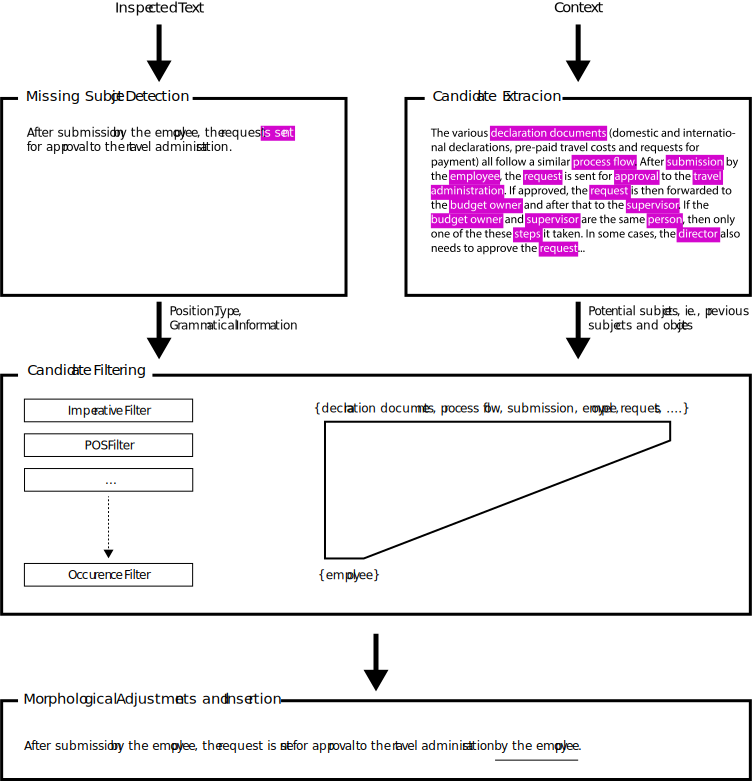
\includegraphics[width=\textwidth]{pipeline}
   \caption{A holistic overview of the pipeline used for implicit subject detection and insertion.}
   \label{fig:pipeline}
\end{figure*}

\subsection{Candidate Extraction}
% not 100% recall but probably only mention in the evaluation.
Candidates are extracted by passing the context through a dependency parser and extracting every word that
appears as either the subject or the object in a phrase. Each word is extracted alongside its dependents.
We can thus differentiate between for example the word `flow' appearing as the head of `the process flow'
or appearing as the head of `a similar flow'. At this stage a very large number of false positives
are provided as well as candidates that we do not want to use, for example due to them being a pronoun
and thus, providing little additional information without a subsequent pass of a coreference resolution
algorithm.


\subsection{Implicit Subject Detection}
For each of the classes mentioned in \ref{methodology:background} distinct extraction rules were developed.

\subsubsection{Passive sentences}
Using a part-of-speech tagger, we can extract verbs in the past participle that have an
auxiliary verb as a dependency. We remove verbs that
already have an agent as a dependency and those that have a subject in the active voice.
Though technically also verbs in the passive voice without subject, we also remove those that
serve as an adverbial modifier as they tend to not take an agent in natural speech.
Further, there exists a set of passive verbs that in general do not take an agent.
For example, the construct `based on' qualifies as a verb in the passive voice without an agent,
but cannot be logically assigned an agent, which we blacklist from extraction.  

\subsubsection{Gerunds}
Similarly, again using a POS tagger, we can directly detect present participles and filter those
out that already have a subject as a dependency. We further prune this set by removing gerunds that
act as adverbial modifiers as their subject are the sentence fragment being modified. 


\subsubsection{(Gerundive) Nouns}\label{detection_gerundive_nouns}
% \cite{pattern_library}
To detect instances of gerundive nominalization, we search for nouns with suffix \textit{-ing}.
We then inspect the stem obtained by removing this suffix. If this stem is in turn a verb, we can
assume the original noun to be a nominalized gerund and be able to take a subject.
Note how we must rely solely on the orthography of the stem. We thus use a predefined list of
English verbs taken from \cite{pattern_library}.
As we will see in the evaluation, this reliance on orthography can cause problems, for example
with homographs.
Note also that this approach may be generalized by using a general stemmer on the inspected noun instead
of only removing the \textit{-ing} suffix. We found this approach to detect too many nouns though.


% evaluation 

% homograph problem

\subsubsection{Imperative}
Imperatives are again easily detected by a POS tagger. We simply filter for verbs in their base
form and disregard those that have an auxiliary verb accompanying them. 



\subsection{Candidate Filtering}\label{filters}
% Mention assembly methods
Conceptually, the candidate filtering can be thought of as a structured ensemble model.
Multiple filtering steps are chained together to produce a final output. In the following,
we will present some possible filters.


\subsubsection{Imperative Filter}
We begin with a simple filter to demonstrate the modus operandi of our filters in general, namely
the imperative filter. If the target detection is an imperative, no elaborate
search must be undertaken as the subject in question is always `you'. Thus, if an imperative
is detected we can filter the list of candidates to only those whose text is `you', creating
a new `you' candidate if needed. If the inspected target is not an imperative we simply
pass on the entire set of candidates to the next filter in the chain. As this filter
has virtually perfect recall, it is best placed at the beginning of the chain.


\subsubsection{Part-of-Speech Filter}
Before taking the context or any semantics into consideration, we further filter the candidates
based on their part-of-speech. More concretely, we disregard candidates that are not nouns.
This filters out mostly pronouns. We argue that we can do this without major loss of information
as the noun referred to by each filtered pronoun should still be present in the context. We do though
loss information on both the quantity and the context with which the candidate entity was referred to
within the text. An alternative would be to apply some form of coreference resolution to replace instead
of simply disregard pronouns. We deem the added complexity to not be worth this marginal information gain.

We make an exception for `you'-candidates and do not filter them as they are needed for imperatives.


\subsubsection{Dependent Of Same Sentence Filter}
Another simple filter that can be applied is disregarding candidates that already act as the object of
the implicit subject construction, specifically those that are already the grammatical subject of
a target predicate in the passive voice. Though technically an entity can be both the grammatical subject and
agent of a verb in the passive voice, in practice such a structure is typically made explicit, for example
through the use of a reflexive pronoun.

\subsubsection{Perplexity Filter}
Oftentimes, a candidate can be disregarded simply from it being semantically incompatible with
the target. For example, when examining the phrase `the house is built' we can exclude
words such as `requirements' and `draft' from consideration as the subject of `built' as they
do not fit semantically, regardless of the given context. We attempt to filter out these words
by using the probability of the sentence with inserted candidate being generated by
a large language model\footnote{We chose GPT-2 \cite{gpt2}, as inference can easily be done on consumer hardware.}.
More accurately, we use the perplexity the model assigns to the candidate sentence \cite{jurafsky}.
To compare different candidates, we examine the ratio of the perplexity of the target sentence
to that of the sentence with the candidate inserted \(\rho\). We found selecting only candidates with
\(\rho \leq 1.5\) to offer a good
tradeoff between selecting too many candidates and filtering out the correct one. A higher ratio
may be picked to filter out fewer candidates and vice versa.



% Evaluation problems with baseline probability

\subsubsection{Similarity Filter}
Another approach is based on the fact that making the implicit subject explicit should not
change the meaning of the sentence. As a consequence, we can rank the candidates by how semantically
similar they are to the original sentence. For this we inspect the cosine similarity of the sentence
embeddings using embeddings generated by Google's Universal Sentence Encoder \cite{universal_sentence_encoder}.


% this straight up does not work.


\subsubsection{Occurrence Filter}
An indication for which candidate is likely to be the most fitting is the candidate's prevalence in
the context. If the candidate occurs often in the context, it is likely to also be relevant for
the target implicit subject. From this we develop a primitive tie breaking mechanism employed at
the end of our pipeline: We simply count the number of times a candidate's text occurs in the
list of candidates and choose the most frequent one. Though not an efficient filter on its own,
it provides better performance than picking a candidate at random at the end of the filter chain.



\subsection{Insertion}\label{insertion}
Though providing only the implicit subject detection and the selected candidate is deemed sufficient for most
% is it?
downstream tasks, implementing an insertion mechanism has both the advantage of creating a full end-to-end
process as well as allowing us to use filter mechanisms that require the candidate to be inserted into
the sentence to assess its relevance. We must preface this by stating that inserting a subject into
a sentence may not have a unique solution.
The sentences `You are fined by the police after 30 days' and `You are fined after 30 days by the police'
are effectively equivalent.
We will discuss the repercussions of this in the evaluation.

For now, we simply focus on creating syntactically and semantically correct sentences. We may again fall
back on our classification of implicit subject types beginning with passive sentences. The goal is
to insert the selected candidate. For this we simply extract the noun chunk of which the candidate is
a part, prefix it with `by' and insert it immediately after the verb. No inflection of the verb is necessary.
In certain situations, we cannot insert the candidate immediately after the verb but rather after
adpositional constructs surrounding the verb. For example, we the phrase
`the data is kept by the controller up to date' though understandable is not as well formed as
`the data is kept up to date by the controller'.
The same insertion mechanism can be used for implicit subjects based on nouns without any adjustments.

Inserting `you' into imperative sentences can be done by inserting the pronoun in front of
verb\footnote{One may argue that additionally inserting a auxiliary verb, e.g., `should',
would capture the semantics of the imperative. We decide against this though to be more inline
with our evaluation data.}. The verb must be inflected to match the second person singular\footnote{The second person
singular is in most cases orthographically equivalent to the imperative. An example exception
is the highly irregular verb `to be'.}. Again, situations may arise where `you' cannot be inserted
immediately preceding the verb. In the case of imperatives this may happen when the verb
appears after an adverbial modifier. If this adverbial modifier is not part of an adverbial clause,
we insert the `you' in front of this adverbial modifier instead. We thus obtain
`[You] \textit{always} select the cheapest parts' but
`\textit{After checking the price}, [you] select the cheapest parts`.

Gerunds can be handled in a very similar way, the only difference being the verb needing to be
inflected according to the number and person of the selected candidate and the candidate being
inserted instead of `you'. We always choose
the present tense for inflection as it is the most fitting for our domain of process descriptions.
Further work is needed to generalize this approach.



%------------------------------------------------------------------------- 
\Section{Evaluation and Discussion}
To evaluate our approach a basic prototype was implemented\footnote{\url{https://github.com/l-rossi/is-with-nlp-implicit-subject}}.
We use Python 3.10 \cite{python} with heavy reliance on the NLP library 
spaCy \cite{spacy} for dependency parsing and POS-tagging. Verb inflection
is based on the pattern library \cite{pattern_library}
The quantitative evaluation was done using a hand-crafter gold standard (73 sentences),
based on a mix of synthetic process descriptions \cite{NLP_bpm_data} and the GDPR \cite{gdpr}.
The inspected text is always a single sentence from each corpus. The context for the process descriptions
is always the entire process description and for the GDPR the entire article from which the inspected sentence
is taken.

\subsection{Quantitative Evaluation}
Our best results were achieved using only a subset of the proposed filters in the following order:
imperative filter, POS filter, dependent of same sentence filter, perplexity filter and occurrence filter.

We conduct two quantitative evaluations targeting first only the implicit subject detection an then
the entire end-to-end pipeline. 
% candidate filter evaluation as its own thing would be nice
Our implicit subject detection mechanism achieves a precision of \(52\%\) at a recall of \(83\%\)
resulting in an F1-score of \(63\%\).
For the end-to-end evaluation we compare each sentence from the gold standard to the generated sentence
by checking if both sentences contain the same tokens with the same dependencies. We match the gold
standard in \(27\%\) of cases.
As we will see in the next subsection, we believe these values to not truly capture the quality
of the pipeline. 

\subsection{Qualitative Evaluation}
A qualitative analysis of the pipeline's outputs will provide a better indication of its strengths
and weaknesses. As little can be said to the candidate extraction step, we group the discussion
thereof with that of the candidate filter step.

\subsubsection{Implicit Subject Detection}
As seen in the quantitative analysis, our detection mechanism has a tendency of detecting more implicit
subjects
than the gold standard. A common problem was the detection of verbs in the passive voice that cannot
logically take an agent, often referred to as `impersonal passive'.
% https://learnenglish.britishcouncil.org/grammar/c1-grammar/advanced-passives-review#:~:text=The%20impersonal%20passive&text=It%20reports%20what%20an%20unspecified,visit%20the%20site%20every%20year.
In the constructs `provided that', referred to in' and `based on' the verb provided cannot take an agent
in any meaningful way. An ad hoc solution would be to blacklist verbs that we know can only appear
in the impersonal passive. There are two major problems with this though. Firstly, maintaining such
a list would be a substantial undertaking and out of the scope of this project. Secondly,
there exist verbs that depending on context can either require the impersonal passive or be
able to take an explicit subject. We thus found no effective way of detecting these
constructs and leave such a task
to future work. A similar thing can happen with certain instances of gerund detections. For example,
the phrase `taking something into account' is a general statement which again cannot take a subject.

In rare cases, the dependency parser employed by us makes minor mistakes. For example, in the sentence
`The information shall be provided by electronic means' the propositional object `by electronic' means
might be identified as an agent instead. In general, the dependency parser is very reliable though and we
see little room for improvement here.

Not all of these detections are strictly erroneous though. Oftentimes it is not clear if a
construct should be amended by a subject or not. An example for this is the sentence
`If approved, the request is then forwarded to the budget owner and after that to the supervisor.'
It is not clear if the second verb `forwarded' should take a subject and if so, which it should be.
Our method detects this as a passive verb in need of a subject, the gold standard though does not
insert a subject here.

A seldomly occurring problem that though highlights some of the limitations of our approach is
that of nouns being detected as nominalized gerunds due to them being homographs of nominalized gerunds.
In our case, the word `evening' has two meanings, the time of day and the nominalized gerund of the verb
`to even'. As our nominalized gerund detection approach only considers orthography, a nonsensical
subject is added to the fragment `in the evening'.


Though false negatives are not considered a major problem of our approach as can be seen from the
comparatively high recall, some interesting observations can still be made. As mentioned in
\ref{methodology:background} we decided to focus on a subset of nouns referring to actions,
namely gerundive nouns. This ignores other nouns referring to actions such as `the withdrawal',
`the renewal', `the omission', etc. As previously mentioned in \ref{detection_gerundive_nouns}
we can generalize our approach to try and include these nouns as well. This though leads
to an unfavorable tradeoff between precision and recall, falling and rising to \(23\%\) and \(88\%\)
respectively. 


\subsubsection{Candidate Selection}
Candidate selection is by far the most challenging part of the pipeline. The most reliable
candidate selection mechanism is that for imperatives, functioning correctly in virtually
every case.
The filter chain can be holistically viewed as first removing obviously false candidates
(Imperative Filter, Part-of-Speech Filter, Dependent of Same Sentence Filter) then trying to
find a semantically viable candidate (Perplexity Filter) and finally narrowing down the
selection to a single candidate by any means possible (Occurrence Filter). Consequently, the first group of
filters tend to cause little problem.

A major drawback of the perplexity filter is its disregard for the wider context of each
inspected target. Filtering is done purely dependent on the probability of a sequence of
tokens being generated by the LLM, which leads to a blatant bias towards rare words. This becomes
apparent with proper nouns which are often disregarded too eagerly. For example, `Blizzard'
in the sentence `[It] starts with \textit{Blizzard} checking whether you have [an] account'
receives \(\rho > 1.7\) although it is the correct candidate.

Though the occurrence filter delivers decent results for such a simple selection mechanism,
its lack of context awareness can lead to naive choices. This problem is exacerbated by
large context sizes as is the case for the articles in the GDPR. A possible solution
would be to use a discounted count of occurrences based on the distance to the target.
One could thereby disregard frequent occurrences of a candidate which are deemed
to be too distant from the currently inspected text. The details of this are
once again left to future work.

Lastly, we would like to discuss the semantic similarity filter, which was not included in
our final pipeline. The filter provided subpar results both when including the context from
the similarity calculations and when excluding it. We believe this to be to the difficulty of
calculating meaningful similarity metrics between large documents and the relative minor effect of
inserting a single subject into these documents. We do believe though, that
this avenue of research is still promising and leave it to future work to find a way of implementing
similarity metrics.




% problems with prior probabilities.

% Group candidate extraction and filtering

% filtering

% Problem with long sentences GDPR <-> synthetic data

\subsubsection{Insertion}
The insertion mechanism is deemed to work close to flawlessly. We only see one
areas of minor improvement, handling verb tense. Luckily for us, in the English
language, the present tense can be used in close to all cases. Nonetheless,
close to all the mismatches caused by the insertion mechanism
between the gold standard and the results from our approach are caused by
a mismatch in tense. Take for example the phrase `when craving'. Our methods
turn this into `when you crave' whereas a technically better match would
be `when you are craving'. This though is a minor mistake which would require
a lot of work to fix and we thus see little room for improvement here.




% TODO what is going on with 42?



%------------------------------------------------------------------------- 
\section{Outlook}
With this project we have provided a framework for solving the problem of detecting
and inserting implicit subjects into text using a rule-based approach. We have provided
sample implementations of each step and provided a prototypical, programmatic implementation
to perform an evaluation of our methods. We do believe that there are still some promising
areas of potential improvements to this approach, namely:

\begin{enumerate}
   \item \textbf{Adding new classes of implicit subjects}: As previously discussed, the
   four classes introduced in this paper are sufficient for describing a majority of
   implicit subject instances. Nonetheless, extending this set of classes may be necessary
   depending on the corpus to which these methods are applied.
   \item \textbf{Widening the class of detected nouns}: We have already demonstrated both
   the need for and an exemplary but insufficient solution to the problem of detecting all
   nouns that can take an implicit subject. This problem is thus still open.  
   \item \textbf{Improving the occurrence filter}: As mentioned in the evaluation section,
   although simply counting the occurrences of each candidate provides a good heuristic for
   the importance of a candidate to the text at large, a more sophisticated approach is deemed
   to offer an avenue of improvement. This could be done either by finding a way of discounting
   each occurrence of a candidate using some metric or instead using more general text summarization
   tools.
   \item \textbf{Improving the similarity filter}: Although we did not manage to make the similarity
   filter perform to a satisfactory degree, we still believe the general idea to hold merit.
   \item \textbf{Impersonal passive voice}: As already discussed, we were not able to detect
   the impersonal passive voice adequately. Consequently, the precision of our pipeline suffers.
   \item \textbf{Incorporating generative AI}: Recent developments have shown the great proficiency
   % sources 
   shown by LLMs when solving NLP tasks. We believe that the capabilities of LLMs to work with semantics
   would complement the more rigid rule-based approach. As a proof-of-concept, our implementation
   contains the possibility of integrating generative AI \cite{openai:2022} in the filter chain (ChatGPTFilter).
   We do this by using the insertion step of
   our pipeline to generate a sentence for each candidate that has not been previously filtered out.
   We then prompt the AI to tell us which of these sentences is the most fitting given the
   user provided context.
   Though this filter does not generally outperform the filters presented in this paper, it shows how one
   may make use of generative AI in a structured manner. Further research into how these two approaches can be combined is thus deemed
   promising.
   % coreference integration?
\end{enumerate}

By combining these improvements with our current approach, we believe we can provide a significant 
contribution to natural language understanding, specifically in the context of business processes.

% previously mentioned improvements
% generative ai


% \nocite{ex1,ex2,ex3}
\bibliographystyle{latex8}
\bibliography{latex8}

\end{document}

